\chapter{Análisis del Sistema}

\begin{abstract}
En este capítulo se aborda el modelado conceptual y funcional del sistema. Tomando como base el catálogo de requisitos y las reglas del dominio definidos previamente en la fase de planificación, se delimita el comportamiento abstracto del sistema de juego mediante el análisis del impacto de sus reglas de negocio y la definición funcional de las interacciones entre los jugadores y la plataforma, omitiendo cualquier condicionante de carácter tecnológico.
\end{abstract}

\section{Trazabilidad del Alcance y Restricciones del Dominio}

El análisis funcional desarrollado en este capítulo se fundamenta de manera directa en el catálogo de requisitos funcionales (RF), requisitos no funcionales (RNF) y reglas de negocio (RN) detallados en la sección 5.1 (Gestión del Alcance) de esta memoria. Con el fin de evitar redundancias y mantener la coherencia metodológica del documento, este apartado se centra exclusivamente en el modelado del sistema desde la perspectiva del problema.

No obstante, la naturaleza asimétrica de \textit{King and Peasant} impone restricciones críticas del dominio que condicionan directamente el comportamiento lógico del sistema. A continuación, se detalla cómo los requisitos de alto nivel del alcance impactan en las reglas lógicas que el sistema debe gobernar:

\begin{itemize}
    \item \textbf{Impacto de la estructura en Eras (RN-01):} Dado que la victoria global exige ganar 2 Eras, el sistema debe ser capaz de contabilizar las victorias acumuladas y orquestar el reinicio completo de los elementos de juego (tablero, mazos y manos) al finalizar una Era, manteniendo la vigencia de la reunión de juego (\textit{Lobby}) sin destruirla.
    
    \item \textbf{Impacto de la capacidad asimétrica (RN-02):} La restricción física del Rey (máximo 3 cartas de Guardia en el \textit{Town}) frente a la capacidad ilimitada del Campesino obliga a que las reglas de validación del sistema apliquen criterios asimétricos dependiendo de la facción del emisor antes de procesar cualquier acción.
    
    \item \textbf{Impacto de la restricción de infiltración (RN-03):} La exigencia de que las cartas objetivo del Campesino estén desplegadas boca abajo en el \textit{Town} para poder activar efectos obliga al sistema a rechazar cualquier intento de infiltración que provenga de la mano o de cartas ya reveladas, blindando el estado lógico del juego.
    
    \item \textbf{Impacto del flujo de turno asimétrico (RN-04):} El robo obligatorio del Rey al finalizar su turno frente al robo voluntario del Campesino exige que el secuenciador de juego sea capaz de inyectar acciones automáticas en la pila de resolución del Rey, manteniendo un sistema de interrupción manual para el Campesino.
    
    \item \textbf{Impacto de la atomicidad de victoria (RN-05):} La asimetría en las condiciones de fin de partida obliga al sistema a evaluar el estado tras cada modificación individual, interrumpiendo cualquier evento encolado si se dispara el criterio de victoria de una facción.
\end{itemize}

\section{Modelado Conceptual y Funcional del Sistema}

Para representar gráficamente la estructura y las interacciones del sistema, se utiliza el Lenguaje Unificado de Modelado (UML), estandarizando la comprensión de la arquitectura lógica y omitiendo, en esta fase, cualquier condicionante de carácter tecnológico o de implementación.

\subsection{Modelo de Dominio Conceptual}

Antes de definir los flujos de interacción de los usuarios, es imperativo establecer el esqueleto estructural del problema y el vocabulario del dominio de \textit{King and Peasant}. En la Fig.~\ref{fig:modelo_dominio} se presenta el Modelo de Dominio Conceptual, el cual abstrae las entidades principales y las reglas de negocio estáticas que rigen el sistema.

El diagrama ilustra una clara separación lógica entre el ecosistema externo de la plataforma y el motor interno del juego. En la capa del sistema, un \textit{Usuario} puede mantener relaciones de amistad con otros y unirse a una \textit{Sala} de espera. Una vez que la \textit{Sala} aloja una \textit{Partida}, el usuario transiciona para actuar bajo la entidad \textit{Jugador}.

Dentro del motor lógico, el modelo refleja de forma rigurosa las asimetrías y restricciones analizadas en la sección anterior. Se observa cómo la \textit{Partida} orquesta el ciclo de vida de hasta tres \textit{Eras}. Los jugadores asumen los roles de \textit{Rey} y \textit{Campesino}, compartiendo zonas de juego comunes como el \textit{Mazo}, el \textit{Descarte} y el \textit{Town}, pero manteniendo su propia \textit{Mano}. Asimismo, la multiplicidad de las relaciones consolida la restricción física crítica del dominio: el \textit{Rey} está limitado a desplegar un máximo de tres cartas de tipo \textit{Guardia} en el \textit{Town}, mientras que el \textit{Campesino} carece de esta limitación al desplegar \textit{Rebeldes}.

\begin{figure}[H]
    \centering
    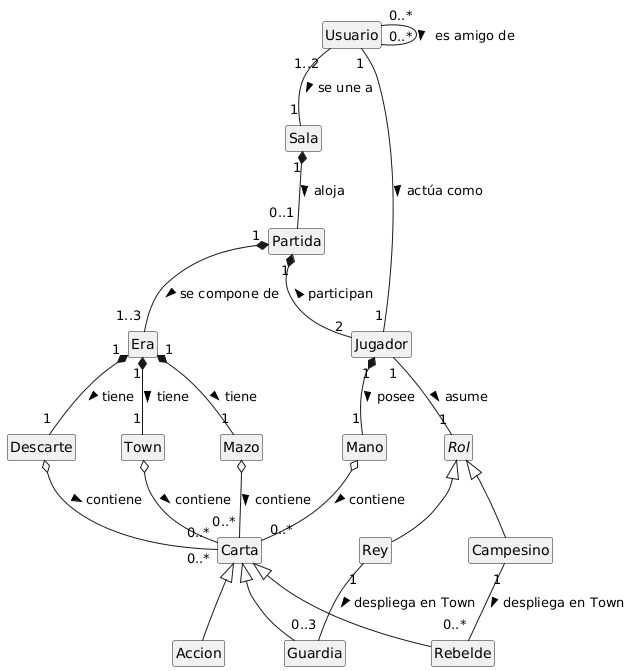
\includegraphics[width=0.9\textwidth]{figures/Modelo_Entidades.png}
    \caption{Modelo de Dominio Conceptual: Entidades lógicas y reglas estructurales del sistema.}
    \label{fig:modelo_dominio}
\end{figure}

\subsection{Diagrama de Casos de Uso}

Una vez definida la estructura estática de la información, en la Fig.~\ref{fig:casos_uso} se detalla el comportamiento dinámico del sistema desde el punto de vista de las funcionalidades ofrecidas. Se observa cómo el \textit{Jugador} tiene la capacidad de acceder al ecosistema central dado que tiene una sesión activa. 

Destaca la modularidad del caso de uso principal (``Jugar Partida''), el cual incluye (\textit{<<include>>}) obligatoriamente la mecánica fundamental de jugar cartas, y se extiende (\textit{<<extend>>}) de forma opcional con acciones accesorias como el chat en vivo o la rendición voluntaria durante el transcurso de la era.

\begin{figure}[H]
    \centering
    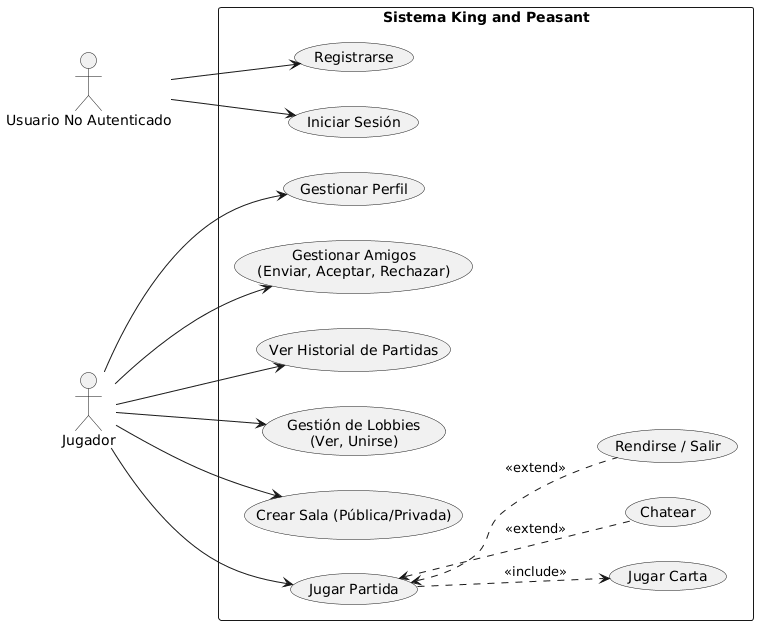
\includegraphics[width=0.8\textwidth]{figures/casos_uso.png}
    \caption{Diagrama General de Casos de Uso del sistema.}
    \label{fig:casos_uso}
\end{figure}

%
%\subsection{Comportamiento Dinámico Conceptual: Flujo de Ejecución}

